\documentclass[conference]{IEEEtran}
\usepackage{pgfplots}
\usepackage{tikz}
\usepackage{amsmath,amssymb,amsfonts}
\usepackage{xcolor}

\begin{document}

  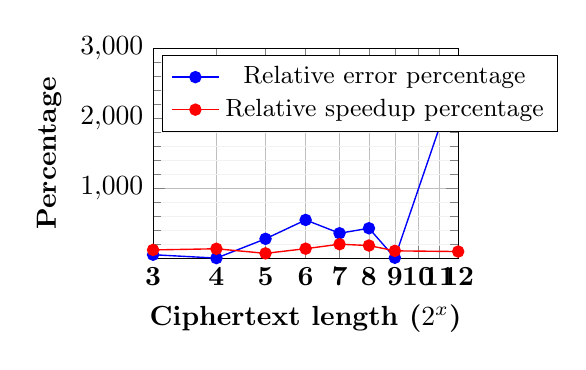
\begin{tikzpicture}
    \begin{axis}[
      width=0.45\textwidth,
      height=0.35\textwidth,
      xlabel={Ciphertext length ($2^x$)},
      ylabel={Percentage},
      font=\bfseries,
      legend pos=north west,
      legend style ={font=\small},
      xmin=3, xmax=12,
      ymin=5, ymax=3000,
      xmode=log,
      xtick={3, 4, 5, 6, 7, 8, 9,10, 11, 12},
      xticklabels={3, 4, 5, 6, 7, 8, 9,10, 11, 12},
      grid=both,
      grid style={line width=.1pt, draw=gray!10},
      major grid style={line width=.2pt,draw=gray!50},
      minor tick num=4,
    ]

es
    \addplot[mark=*, blue, line width = 0.5pt] table[x=Ciphertext, y=Error] {
      Ciphertext Error
        3 54.0085
        4 5.56393
        5 280.867
        6 550.884
        7 360.715
        8 431.906
        9 10.2816
        12 2655.09
    };
    \addlegendentry{Relative error percentage}

    \addplot[mark=*, red, line width = 0.5pt] table[x=Ciphertext, y=Speedup] {
      Ciphertext Speedup
        3 122.245
        4 138.9
        5 73.406
        6 140.216
        7 203.902
        8 185.171
        9 109.212
        12 99.2016
    };
    \addlegendentry{Relative speedup percentage}
    % Scatter plots and lines

    \end{axis}
  \end{tikzpicture}

\end{document}